\documentclass{beamer}
\usetheme{Warsaw}
\useinnertheme{circles}
\useoutertheme[subsection=false]{smoothbars}
\usepackage[utf8x]{inputenc}
\usepackage[czech]{babel}
\usepackage[T1]{fontenc}
\usepackage{listings}
\usepackage{tikz}
\lstset{basicstyle=\tiny\ttfamily}
\logo{
\includegraphics[height=0.5cm]{brmlab.pdf}}

\begin{document}

\AtBeginSection[]
{
  \begin{frame}
    \frametitle{Outline}
    \tableofcontents[currentsection]
  \end{frame}
}

\title{brmiversity: Umělá inteligence \\ a teoretická informatika}
\subtitle{Přednáška č. 4}
\author{Petr Baudiš $\langle${\tt pasky@ucw.cz}$\rangle$}
\institute{
	brmlab 2011\\
	\vskip 1ex
	\pgfdeclareimage[height=4ex]{ccbysa}{by-sa.pdf}
	\pgfuseimage{ccbysa}
}
\date{}
\frame{\titlepage}

\section{Neuronové sítě}

\subsection{}
\begin{frame}{Umělá neuronová síť}
\begin{itemize}
\item Jednoduché schéma
\end{itemize}
\end{frame}

\subsection{}
\begin{frame}{Perceptron}
\begin{itemize}
\item Diagram, základní vzoreček, obrázek roviny
\end{itemize}
\end{frame}

\subsection{}
\begin{frame}{Co dokáže perceptron?}
\begin{itemize}
\item Lineární separabilita
\item Omezení --- XOR
\end{itemize}
\end{frame}

\subsection{}
\begin{frame}{Geometrická interpretace}
\begin{itemize}
\item Váhový vektor v rovině
\end{itemize}
\end{frame}

\subsection{}
\begin{frame}{Učení perceptronu}
\begin{itemize}
\item ``Rotační'' algoritmus
\end{itemize}
\end{frame}

\subsection{}
\begin{frame}{Otázky?}
\begin{center}
Příště: Vícevrstvé neuronové sítě a jejich učení (backpropagation).
\end{center}
\end{frame}

\section{Umělá inteligence}

\subsection{}
\begin{frame}{Filosofie}
\begin{itemize}
\item Silná vs. slabá AI
\item AI-complete úlohy
\item Bude víc 23.11.
\item Dnes jeden příklad slabé AI (je AI-complete?)
\end{itemize}
\end{frame}

\subsection{}
\begin{frame}{Matematické hry}
\begin{itemize}
\item Teorie her --- hráči se střídají v akcích, každý dostane nějakou výplatu po dokončení sekvence akcí
\item Hry dvou hráčů s úplnou informací a nulovým součtem
\end{itemize}
\end{frame}

\subsection{}
\begin{frame}{Minimaxový strom}
\begin{itemize}
\item ``Adversarial planning''
\item Tah je tak dobrý jako nejnepříjemnější tah protihráče
\item Omezení na hloubku stromu --- vyhodnocovací funkce
\end{itemize}
\begin{center}
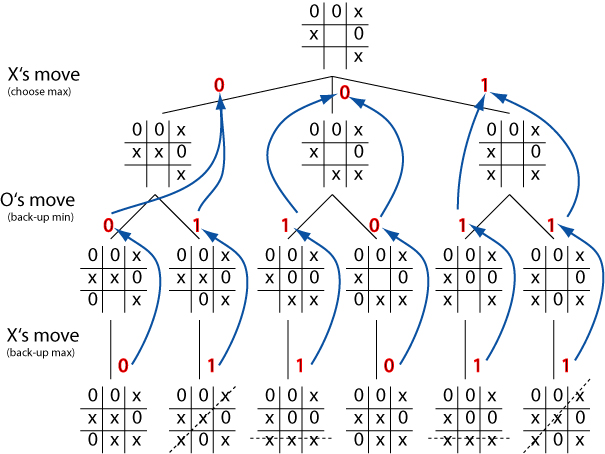
\includegraphics[width=7cm]{minimax-illustration.jpg}
\end{center}
\end{frame}

\subsection{}
\begin{frame}{$\alpha,\beta$ prořezávání}
\begin{itemize}
\item Základní urychlovací heuristika
\item Pamatujeme si nejhorší a nejlepší hodnoty z minimaxových sousedů, zařízneme prohledávání uzlu, je-li jasné, že bude horší (max, $\alpha$) nebo lepší (min, $\beta$)
\item Pro efektivitu je důležité pořadí vyhodnocování tahů
\end{itemize}
\begin{center}
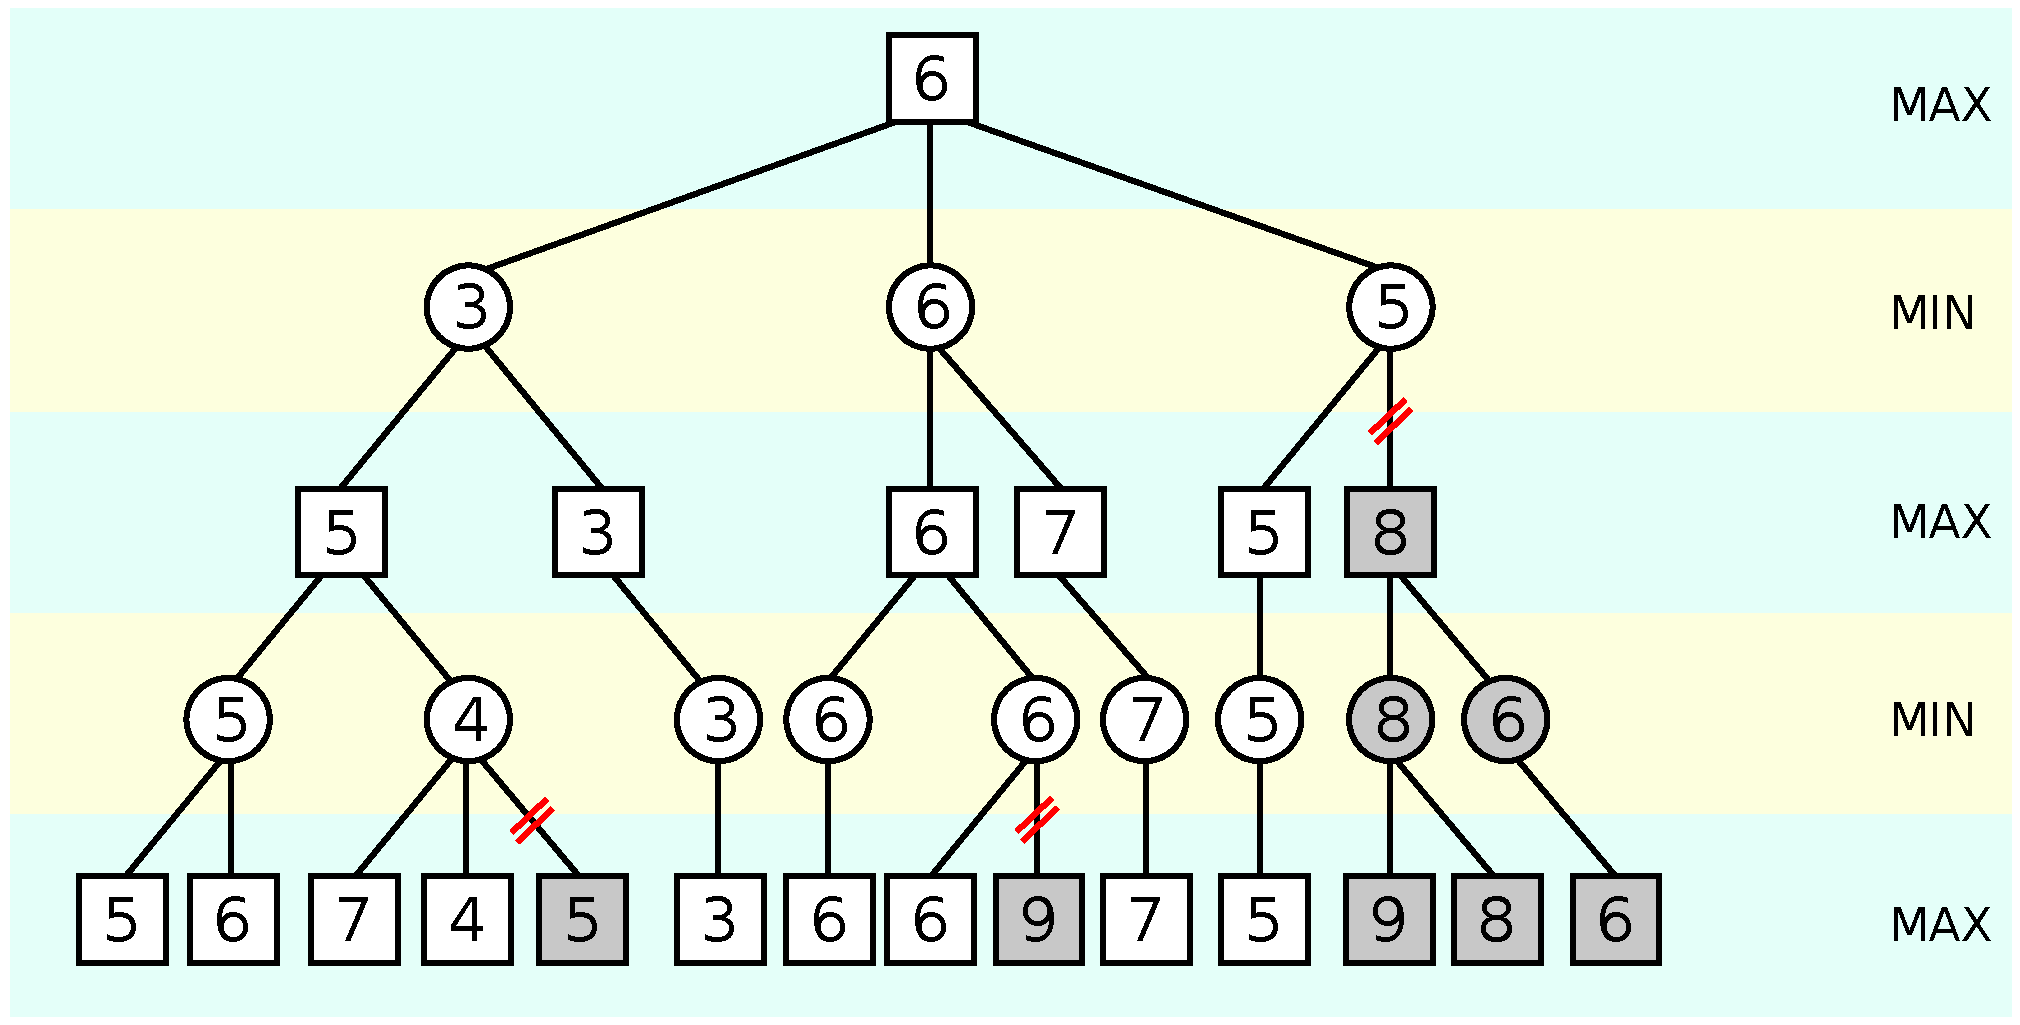
\includegraphics[width=6cm]{AB_pruning.pdf}
\end{center}
\end{frame}

\subsection{}
\begin{frame}{Další vylepšení}
\begin{itemize}
\item Transpoziční tabulky
\item Prořezávání, singular extensions, atd.
\item Problémy --- dobrá funkce, větvící faktor, efekt horizontu
\end{itemize}
\end{frame}

\subsection{}
\begin{frame}{Monte Carlo Tree Search}
\begin{itemize}
\item Technika Monte Carlo
\item Minimaxový strom s očekáváními
\item Multi-armed bandit
\end{itemize}
\begin{center}
\includegraphics[width=8cm]{mcts.png}
\end{center}
\end{frame}

\subsection{}
\begin{frame}{Otázky?}
\begin{center}
Příště: Prohledávání v grafech.
\end{center}
\end{frame}

\section{Základní algoritmy}

\subsection{}
\begin{frame}{Levenšteinova editační vzdálenost}
\begin{itemize}
\item Dva stringy; editace jsou přidání, změna, odebrání
\item Dynamický algoritmus:
\end{itemize}

\begin{center}
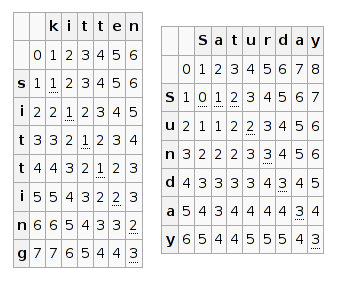
\includegraphics[width=6cm]{levehnstein.png}
\end{center}
\end{frame}

\subsection{}
\begin{frame}{Další způsoby porovnávání}
\begin{itemize}
\item Myersův algoritmus (nejdelší společná podposloupnost \\ neboli editační skript; jen $+$ a $-$)
\item bdiff (nejdelší společný podřetězec --- rekurzivně)
\item xdelta (rsync; Rabinovo hashování)
\end{itemize}
\end{frame}

\section{Složitost}

\subsection{}
\begin{frame}{Metody tvorby algoritmů}
\begin{itemize}
\item Kuchařka pro efektivní algoritmy na obecné třídy problémů
\item Rozděl a panuj --- problém rozdělíme na podproblémy \\ a ty počítáme rekurzivně
\item Hladový algoritmus --- problém budujeme inkrementálně, v~každé chvíli víme, kudy dál
\item Dynamický algoritmus --- problém budujeme inkrementálně, sdílíme výsledky jednodušších podproblémů
\end{itemize}
\end{frame}

\subsection{}
\begin{frame}{Rozděl a panuj --- příklad}
\begin{itemize}
\item Binární vyhledávání: \\
	\only<1>{1 3 9 10 12 13 17 19 24 26 27 30 31}
	\only<2>{1 3 9 10 12 13 {\bf 17} 19 24 26 27 30 31}
	\only<3>{1 3 9 10 12 13 {\tiny 17 19 24 26 27 30 31}}
	\only<4>{1 3 {\bf 9} 10 12 13 {\tiny 17 19 24 26 27 30 31}}
	\only<5>{{\tiny 1 3 9} 10 12 13 {\tiny 17 19 24 26 27 30 31}}
	\only<6>{{\tiny 1 3 9} 10 {\bf 12} 13 {\tiny 17 19 24 26 27 30 31}}
	\only<7>{{\tiny 1 3 9} 10 {\tiny 12 13 \tiny 17 19 24 26 27 30 31}}
\item Quicksort
\end{itemize}
\end{frame}

\subsection{}
\begin{frame}{Master Theorem}
\begin{itemize}
\item Asymptotická složitost?
\end{itemize}
\end{frame}

\subsection{}
\begin{frame}{Hladový algoritmus --- příklad}
\begin{itemize}
\item Minimální kostra (připomenutí)
\item Rozvrhovací problém
\item Dijkstra
\end{itemize}
\end{frame}

\subsection{}
\begin{frame}{Matroidy}
\begin{itemize}
\item Hladový algoritmus lze použít, pokud problém vykazuje {\em optimální podstrukturu}
\item Matematická abstrakce
\end{itemize}
\end{frame}

\subsection{}
\begin{frame}{Dynamický algoritmus}
\begin{itemize}
\item Editační vzdálenost
\item Fibonacciho posloupnost
\item Dijkstra
\vskip 3ex
\item Optimální podstruktura a překrývající se podproblémy
\end{itemize}
\end{frame}

\subsection{}
\begin{frame}{Třídění}
\begin{itemize}
\item Jak dlouho trvá třídění? $O(n\cdot\log n)$
\item Vyhledávací strom
\item Proto nejde třídit rychleji
\item Nebo ano? Radix sort, ale je to podvod!
\end{itemize}
\end{frame}

\subsection{}
\begin{frame}{Otázky?}
\begin{center}
Příště: Pravděpodobnostní algoritmy.
\end{center}
\end{frame}

\section{Vyčíslitelnost}

\subsection{}
\begin{frame}{Rekapitulace}
\begin{itemize}
\item Rekapitulace: Nezajímá nás, jak rychle to poběží, \\ ale jestli to někdy doběhne.
\item Zkoumáme výpočetní {\em možnosti} algoritmů.
\vskip 3ex
\item Minule jsme přemýšleli, čím vším lze algoritmy vykonávat \\ (a že je to ekvivalentní).
\item Zapomněli jsme (mj.) na {\bf celulární automaty}! % TODO: obrazek
\end{itemize}
\end{frame}

\subsection{}
\begin{frame}{Halting Problem}
\begin{itemize}
\item Máme program $z=x(y)$; $x, y, z$ jsou čísla \\ (kód, parametr / vstup, návratová hodnota / výstup)
\item Program doběhne (v konečném čase) a vrátí hodnotu \\ ({\em řeší} problém), nebo se zacyklí
\pause
\vskip 3ex
\item Nekonečná smyčka v závislosti na datech, \\ schovaná uprostřed složitého kódu
\item Halting Problem: Zacyklí se program $x$ na vstupu $y$?
\item Dokážeme napsat program, který řeší halting problem?
\end{itemize}
\end{frame}

\subsection{}
\begin{frame}{Halting Problem: Důkaz}
\begin{itemize}
\item PODRAZ
\end{itemize}
\end{frame}

\subsection{}
\begin{frame}{Otázky?}
\begin{center}
Příště: Rekurzivní a rekurzivně spočetné množiny.
\end{center}
\end{frame}

\subsection{}
\begin{frame}{Děkuji vám}
\begin{center}
{\bf pasky@ucw.cz}

\vskip 6ex

Příště: {\bf Nebude.}

\vskip 6ex

Popříště: Prohledávání grafů a hledání cesty (základní algoritmy, umělá inteligence, adaptivní agenti), neuronové sítě, vyčíslitelnost.
\end{center}
\end{frame}

\end{document}
